\documentclass[12pt]{article}
\usepackage{amsmath,amssymb}
\usepackage{geometry}
\usepackage{enumitem}
\usepackage{tikz}
\geometry{margin=0.85in}

\newcommand{\graphgrid}{%
\begin{center}
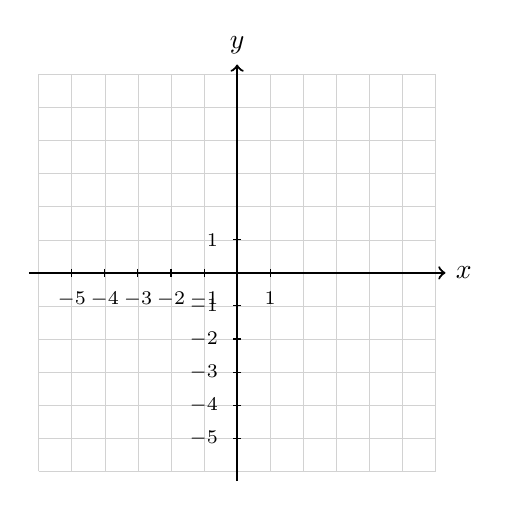
\begin{tikzpicture}[scale=0.42]
  \draw[step=1cm,gray!35,very thin] (-6,-6) grid (6,6);
  \draw[->,thick] (-6.3,0)--(6.3,0) node[right] {$x$};
  \draw[->,thick] (0,-6.3)--(0,6.3) node[above] {$y$};
  \foreach \x in {-5,...,-1,1,...,5} \draw (\x,0.12)--(\x,-0.12) node[below=2pt] {\scriptsize $\x$};
  \foreach \y in {-5,...,-1,1,...,5} \draw (0.12,\y)--(-0.12,\y) node[left=2pt] {\scriptsize $\y$};
\end{tikzpicture}
\end{center}}

\title{Algebra I Readiness Review for Algebra II Honors}
\author{}
\date{}

\begin{document}
\maketitle

\section*{Instructions}
Complete in 45 minutes. Show clear algebraic work and check solutions when possible. Give exact answers using fractions and radicals; do not use rounded decimals. This review covers foundational skills expected at the beginning of Algebra II Honors.

\section*{Quick Reference}
\[
  m=\frac{y_2-y_1}{x_2-x_1},
  \qquad y-y_1=m(x-x_1),
  \qquad y=mx+b
\]
\[
  a^ma^n=a^{m+n},
  \qquad \frac{a^m}{a^n}=a^{m-n},
  \qquad (a^m)^n=a^{mn}
\]
\[
  x=\frac{-b\pm\sqrt{b^2-4ac}}{2a},
  \qquad
  (a+b)^2=a^2+2ab+b^2,
  \qquad
  a^2-b^2=(a-b)(a+b)
\]

\section*{Problems}
\begin{enumerate}[leftmargin=*,itemsep=1.2em]
  \item Simplify completely:
  \[
    4(2x-3)-3(x+5)+2(1-2x).
  \]

  \item Solve and check:
  \[
    \frac34(2x-8)-\frac13(x+6)=5.
  \]

  \item Solve each inequality. Write each answer in interval notation.
  \begin{enumerate}[label=(\alph*),itemsep=0.4em]
    \item $5-3(2x-1)>4x+8$
    \item $|2x-5|\le9$
  \end{enumerate}

  \item The points $(-2,5)$ and $(4,-1)$ lie on line $\ell$.
  \begin{enumerate}[label=(\alph*),itemsep=0.4em]
    \item Find the slope of $\ell$ and write its equation in slope-intercept form.
    \item Write the equation of the line parallel to $\ell$ through $(3,-4)$.
  \end{enumerate}

  \item Let $f(x)=x^2-4x+1$.
  \begin{enumerate}[label=(\alph*),itemsep=0.4em]
    \item Find $f(-3)$.
    \item Solve $f(x)=1$.
    \item Find the average rate of change of $f$ from $x=1$ to $x=5$.
  \end{enumerate}

  \item Solve the system exactly:
  \[
    \begin{cases}
      2x+3y=7,\\
      4x-y=5.
    \end{cases}
  \]

  \item Simplify completely. Use positive exponents and rationalize denominators.
  \begin{enumerate}[label=(\alph*),itemsep=0.5em]
    \item $\displaystyle \left(\frac{6x^{-2}y^3}{3xy^{-1}}\right)^2$
    \item $\sqrt{72}-2\sqrt8+\sqrt{18}$
    \item $\displaystyle \frac5{2-\sqrt3}$
  \end{enumerate}

  \item Perform the indicated operations and simplify.
  \begin{enumerate}[label=(\alph*),itemsep=0.5em]
    \item $(2x-3)(x^2+x-4)$
    \item Divide $2x^3-3x^2-11x+6$ by $x-3$.
  \end{enumerate}

  \item Factor completely over the integers.
  \begin{enumerate}[label=(\alph*),itemsep=0.5em]
    \item $2x^2-7x-15$
    \item $x^3-4x^2-x+4$
    \item $9y^2-25$
  \end{enumerate}

  \item Solve exactly.
  \begin{enumerate}[label=(\alph*),itemsep=0.5em]
    \item $2x^2-3x-5=0$
    \item $x^2-6x+2=0$
    \item $3x^2=27$
  \end{enumerate}

  \item For $y=-x^2+4x+5$:
  \begin{enumerate}[label=(\alph*),itemsep=0.4em]
    \item Find the vertex, axis of symmetry, and intercepts.
    \item State the domain and range.
    \item Graph the function on the coordinate plane.
  \end{enumerate}
  \graphgrid

  \item A rectangle has an area of $96$ square feet. Its length is 4 feet greater than its width.
  \begin{enumerate}[label=(\alph*),itemsep=0.4em]
    \item Write a quadratic equation that models the situation.
    \item Find the rectangle's dimensions.
    \item If both dimensions are increased by 25\%, by what percent does the area increase?
  \end{enumerate}
\end{enumerate}

\end{document}
